\chapter{Problem description} \label{chap::problem}
{\it \centering In this chapter, the impact-based SLAM problem is described from a probabilistic viewpoint in Section~\ref{sec::formulation}. The essentials for building an accurate SLAM solution are a robot motion model and an environment representation. Section~\ref{sec::robotmodel} details the various motion models for the SLAM problem suitable for specific scenarios. Various environment representations suitable for rectilinear environments are discussed in Section~\ref{sec::env_rep} along with the proposed histogram maps. Section~\ref{sec::challenges} addresses various challenges relevant to the impact-based SLAM problem.}

\section{Notations}
In the impact-based SLAM problem, the Sphero robot collides with the walls of a given rectilinear environment randomly. The collision information, along with odometry through dead-reckoning, from the robot can infer the pose of a landmark. The odometry gives the position of collision while the collision information is used for calculation of landmark orientation. The collision is detected in Sphero when there is a sudden deceleration in either or both of the robot's coordinate axes X and Y. The wall orientation $\phi$ can be inferred from the collision information with respect to the robot's orientation \gsymb{$\theta$}{Robot orientation} by measuring the change or peak of impact along each coordinate axis. The dependence is shown below,
\begin{equation}
\phi-\theta = \arctan\left(\frac{a_x}{a_y}\right),
\end{equation}
where $a_x$ and $a_y$ represent the accelerometer reading at the highest peak of impact or the power of impact along the coordinate axis X and Y respectively. Further information about collision detection can be found in Section~\ref{sec::sphero} of Chapter \ref{chap::implementation}. 

At time instant \textit{t}, following quantities are defined:
\begin{description}
\item[$s_t:$] pose of the robot, containing position and orientation information
\item[$u_t:$] control input vector, containing velocity and heading, applied at time instant $\textit{t}-1$ to get the pose $s_t$
\item[$m_i:$] $i^{th}$ landmark position or pose
\item[$c_t:$] measurement correspondence at time $t$
\item[$z_t:$] measurement/observation from robot at time $t$
\end{description}

The time history of a variable $s$ is denoted as $s_{0:t}$. The correspondence of a landmark to an incoming measurement is called as data association and it is crucial for any SLAM problem. This step is very important since standard estimators are prone to divergence for incorrect associations.

\section{Probabilistic formulation}  \label{sec::formulation}
The probabilistic formulation of the SLAM describes the problem in the most certain way possible with uncertainty dealt explicitly. The uncertainty in the SLAM problem, crucial for tractability, has been modelled in few of the most common forms. For example, in the case of Extended Kalman filter, the uncertainty is modelled as a Gaussian while the particle filter models the uncertainty as a set of particles.

There are two main forms of the probabilistic SLAM problem, which are equally important in their own aspects and have their own pros and cons. One is known as the online SLAM problem, involving estimation of posterior over momentary pose along with the map. The online version is an incremental algorithm which discards past measurements and controls once they have been processed. Using the above notations, online SLAM is defined as the following posterior:
\begin{equation}
p(s_t,m|z_{1:t},u_{1:t},c_{1:t})
\end{equation}
If the set of data associations is known, the posterior becomes simple: 
\begin{equation}
p(s_t,m|z_{1:t},u_{1:t})
\end{equation}

A convenient way to describe a probabilistic SLAM algorithm and its structure is through a \ac{DBN}. Expressing SLAM through a DBN highlights its temporal structure as a Markov chain. A Bayesian network is a graphical model describing a stochastic process as a directed graph. The graph has one node for each variable in the process and a directed edge between two nodes models the conditional dependence between them. For further information on Bayesian networks, refer \cite{koller2009probabilistic}. For example, the online SLAM problem as a DBN is depicted in Figure~\ref{online_SLAM}. 

\begin{figure}
\centering
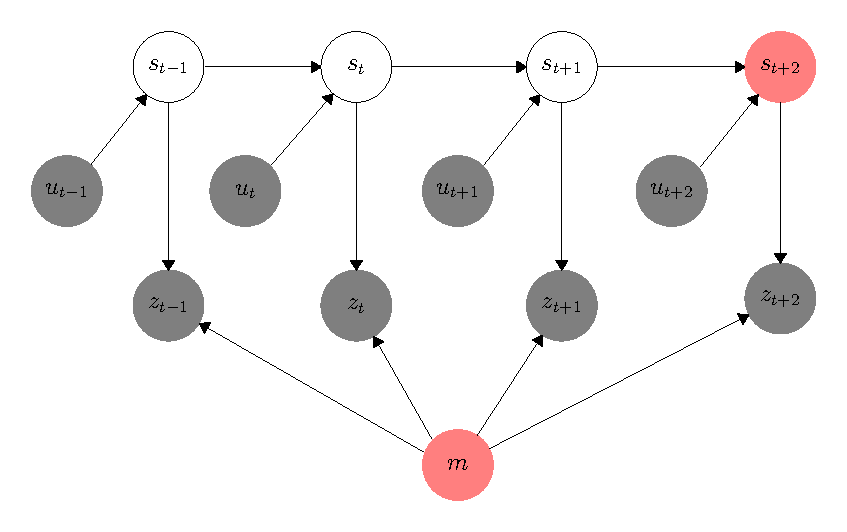
\includegraphics[scale=0.9]{./images/fsm2}
\caption[Dynamic Bayesian Network graph of online SLAM problem]{Graphical model of online SLAM problem. The online SLAM estimates a posterior over the current robot pose and map. The red shaded nodes are estimated in this problem given the gray shaded nodes.}
\label{online_SLAM}
\end{figure}

\begin{figure}
\centering
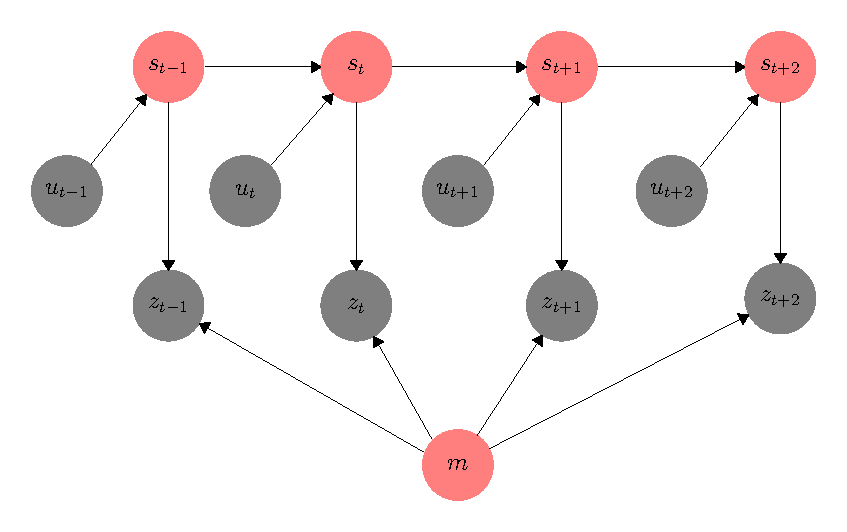
\includegraphics[scale=0.9]{./images/fsm3}
\caption[Dynamic Bayesian Network graph of full SLAM problem]{Graphical model of full SLAM problem. The full SLAM estimates a posterior over the entire robot trajectory and map. The red shaded nodes are estimated in this problem given the gray shaded nodes.}
\label{full_SLAM}
\end{figure}

The other form of probabilistic SLAM is called full SLAM problem which calculates the posterior over the entire pose trajectory along with the map. The data association set is assumed to be known.
\begin{equation}
P(s_{1:t},m|z_{1:t},u_{1:t})
\end{equation}

The full SLAM problem as a DBN is depicted in Figure~\ref{full_SLAM}. The initial condition $s_0$ is assumed to be known in both the SLAM forms and is removed from the conditioning term for simplicity in notations.

The full version of the SLAM problem involves the entire measurement and state information which results in an enormous computational complexity introduced by the huge data, while the online version is more suitable for practical applications such as navigation since the measurements are processed as they arrive. However, the full SLAM results in a more accurate and consistent estimate since it models the entire set of correlations between the measurements and robot trajectory which is neglected in the online version.

In general, a recursive solution to the SLAM problem is desirable since measurements can be processed as they arrive. The joint posterior is updated using Bayes' Theorem with the help of a state transition model and an observation model which are individually affected by control input and observation respectively. 

A state transition model describes a systematic update to the pose of the robot in terms of a probability distribution of the form-
\begin{equation}
P(s_t|s_{t-1},u_t).
\end{equation} 

The state transition model is assumed to be a Markov process in which the next state of the robot depends only upon the previous robot pose and recent control action. This structure is important for reducing the computational complexity of the SLAM problem.  

The observation model describes the probability of making an observation given the robot pose and map of the environment- 
\begin{equation}
P(z_t|s_t,m).
\end{equation}

If the landmark is a new one, it has to be appended to a set of new landmarks. The landmark initialization function is defined as the inverse of observation model. 

The state transition model and observation model characterizes the connectivity of the Bayesian network through a recurrent pattern as shown in Figures~\ref{online_SLAM}~and~\ref{full_SLAM}. The state transition model is represented by the edges connecting the state variable which represents the probability of state variable at that time instant. Similarly, the observation model models the probability of performing an observation given that the robot is at a location in the map. Expressing SLAM as DBN highlights its temporal structure, and this formalism is exclusively suited to describe SLAM as a filtering problem. 

The recursive Bayesian update is carried out using the state transition and observation model in a two-step recursive procedure, more popularly called as Bayes filter. The Bayes filter can be derived from the SLAM posterior as follows.

\textbf{Bayes filter derivation}

The SLAM posterior can be rewritten using the Bayes' rule as given below.
\begin{equation}
p(s_t,m|z_{1:t},u_{1:t},c_{1:t}) = \eta\cdot p(z_t|s_t,m,z_{1:t-1},u_{1:t},c_{1:t})\cdot p(s_t,m|z_{1:t-1},u_{1:t},c_{1:t})
\end{equation}

The first term in the product, $\eta$, is a normalizing constant in the Bayes' rule. The fact that the current measurement $z_t$ is solely a function of pose of the robot $s_t$, map $m$ and data association $n_t$ can be exploited to simplify the above product. 
\begin{equation}
p(s_t,m|z_{1:t},u_{1:t},c_{1:t}) = \eta\cdot p(z_t|s_t,m,,c_{1:t})\cdot p(s_t,m|z_{1:t-1},u_{1:t},c_{1:t})
\end{equation}

Using the theorem of total probability to condition the last term of the product on pose at time $t-1$,
\begin{equation}
= \eta\cdot p(z_t|s_t,m,c_{1:t})\cdot\int p(s_t,m|s_{t-1},z_{1:t-1},u_{1:t},c_{1:t})\cdot p(s_{t-1}|z_{1:t-1},u_{1:t},c_{1:t})\cdot ds_{t-1}
\end{equation}

The leftmost term in the integral can be expanded using conditional probability theory.
\begin{equation}
\begin{split}
= \eta\cdot p(z_t|s_t,m,,c_{1:t})\cdot\int p(s_t|m,s_{t-1},&z_{1:t-1},u_{1:t},c_{1:t})\cdot p(m|s_{t-1},z_{1:t-1},u_{1:t},c_{1:t})\cdot \\
&\cdot p(s_{t-1}|z_{1:t-1},u_{1:t},c_{1:t})\cdot ds_{t-1}
\end{split}
\end{equation}

The first term of the above product can be simplified assuming the state propagation is a Markov process, hence $s_t$ is only a function of $s_{t-1}$ and $u_t$. 
\begin{equation}
\begin{split}
= \eta\cdot p(z_t|s_t,m,,c_{1:t})\cdot\int p(s_t|s_{t-1},u_t)&\cdot p(m|s_{t-1},z_{1:t-1},u_{1:t},c_{1:t})\cdot \\
&\cdot p(s_{t-1}|z_{1:t-1},u_{1:t},c_{1:t})\cdot ds_{t-1}
\end{split}
\end{equation}

Also, the last two terms in the integral product can be combined together using Bayes' product.
\begin{equation}
\begin{split}
p(s_t,&m|z_{1:t},u_{1:t},c_{1:t}) = \\
&\eta\cdot p(z_t|s_t,m,,c_{1:t})\cdot\int p(s_t|s_{t-1},u_t)\cdot p(s_{t-1}, m|z_{1:t-1},u_{1:t},c_{1:t})\cdot ds_{t-1}
\end{split}
\end{equation}

Since the process is causal in such a way where the current input $u_t$ and data association $c_t$ provide no new information about the previous state $s_{t-1}$ or map m without the latest observation $z_t$, they can be dropped from the rightmost term of the integral. The result obtained turns out to be a recursive formula for computing the SLAM posterior at time $t$ given the SLAM posterior at time $t-1$, motion model $p(s_t|s_{t-1},u_t)$ and observation model $p(z_t|s_t,m,c_t)$.

The state transition probability assumes a Markov propagation in system states for computational efficiency. The Markov assumption states that the probability distribution of the next state depends upon the previous state and not on the sequence of states that preceded it. This requires a crucial assumption that the system is characterized by a complete state.
\begin{defn}
A complete state is defined as a characterization of a system which can be the best predictor of the future. If any state is sufficient to describe a future state with a given input, the past states can be neglected in calculations.
\label{def1}
\end{defn} 

The error from the latter can be compensated by inflating the covariance information of the corresponding process. This assumption is quite successful in practical SLAM algorithms, especially in particle filter-SLAM algorithm where the pose error is factored out. The problem in the former case can be removed by considering a modified complete state of the system.

The accuracy of the prediction step is increased by conditioning the map state in state transition probability $p(s_t|s_{t-1},u_t,m)$. Inclusion of map state tends to remove poor state hypotheses in Bayes filter. A similar statement is used in the particle filter-SLAM algorithm where measurements are included in the prediction step to reduce degeneracy of particle filter. However, computation of this probability can be cumbersome and efficient approximations are used. Let us briefly derive it using Bayes' rule.
\begin{equation}
p(s_t|u_t,s_{t-1},m)\cdot p(m|u_t,s_{t-1}) = p(m|s_t,u_t,s_{t-1})\cdot p(s_t|u_t,s_{t-1})
\end{equation}

As $p(m|u_t,s_{t-1})$ can be considered a constant $\eta$, a desired approximation of $p(m|s_t,u_t,s_{t-1})$ is used as $p(m|s_t)$.
\begin{equation}
p(s_t|u_t,s_{t-1},m) = \eta\cdot p(m|s_t)\cdot p(s_t|u_t,s_{t-1})
\end{equation}

A similar Bayes' rule product is obtained with a different normalization constant $\hat{\eta}$.
\begin{equation}
p(s_t|u_t,s_{t-1},m) = \hat{\eta}\cdot p(s_t|m)\cdot p(s_t|u_t,s_{t-1})
\end{equation}

Inclusion of $p(s_t|m)$ can improve the accuracy of the prediction step through reduced degeneracy. For example, as the robot comes close to a wall, it is not good to represent a probability of robot being present on the wall or the other side. Hence, an inclusion of map can remove this problem. A detailed proof of the modified prediction step or proposal distribution is provided in Appendix~\ref{mod_prop}.  

Various SLAM algorithms quite differ on the representation of these probability distributions and type of the sensors used. The following sections describe these distributions that are suitable for the impact-based SLAM. The importance and manipulation of these recursive steps will be explained in detail in future.

\section{Robot model} \label{sec::robotmodel}
The goal of a probabilistic robot model is to accurately model the specific types of uncertainty that exists in robot actuation and perception. In practice, the exact model seems to be less important than the fact that some provisions for uncertain outcomes are provided in the first place. Accurately modelling the robot is important to control the robot dynamics but in situations where certain dynamics of the robot are not excited much as part of the problem, it is not useful to model them. For the impact-based SLAM, the Sphero robot moves in straight lines between collisions and rotates around itself at the collision point.  Hence, a unicycle model is sufficient to explain the behaviour of this motion and the unmodeled dynamics can be accounted as uncertainty. In case of motion planning, more accurate geometric models such as SO(3) are needed and will be considered as future work of this thesis.

\subsection{Motion model}
There are two specific probabilistic motion models for the Sphero mobile robot. Both the models are somewhat complimentary in the type of motion information being processed. The first model, called velocity motion model, assumes that the motion data specifies the velocity and heading commands given to the robot. The second model, called odometry motion model, assumes that the motion information is provided through the odometry. The latter is more accurate than the former for a simple reason that error in the unmodelled robot kinematics are not accounted  and the information is available post-the-fact. The velocity motion model is most suitable for autonomous robots as it incorporates the robot motion model which is essential for motion planning. 

The two models used in SLAM algorithms are shown in Figures~\ref{vel_model}~and~\ref{odom_model}. 

\begin{figure}
\centering
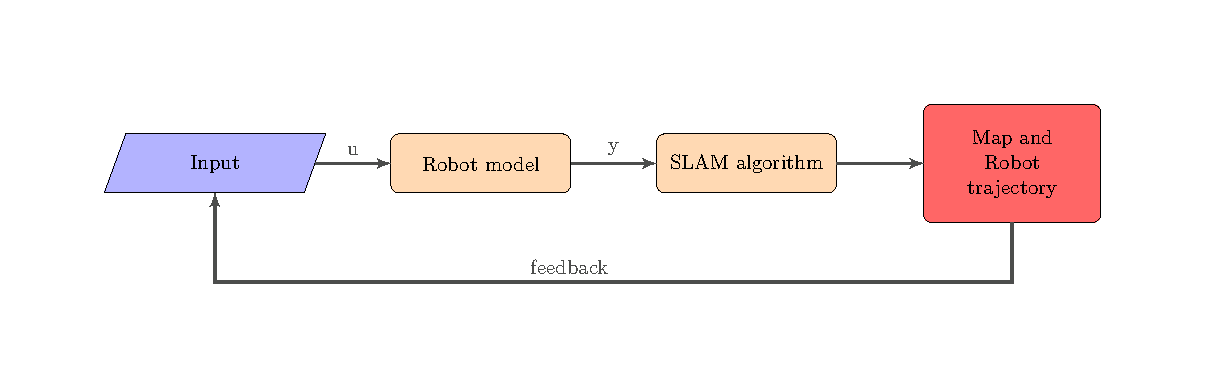
\includegraphics[scale=0.75]{./images/vel_model}
\caption[Velocity model]{Velocity model for SLAM with planning; $\text{u}$ denotes control input and y denotes the measurement including the odometry. The feedback enables planning in SLAM.}
\label{vel_model}
\end{figure}

\begin{figure}
\centering
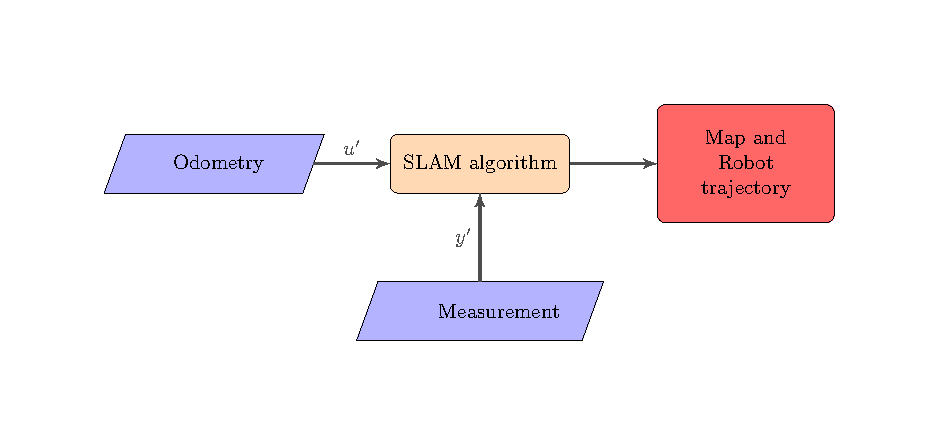
\includegraphics[scale=0.75]{./images/odom_model}
\caption[Odometry model]{Odometry model for SLAM; $u'$ denotes odometry input and $y'$ denotes the collision measurement}
\label{odom_model}
\end{figure}

\subsubsection{Velocity motion model}
A sampling based approach is used to compute the state transition probability from a given state $s_{t-1}=[x_{t-1},y_{t-1},\phi_{t-1}]$ and control input $[\text{speed},\text{head}]$. The time from $t-1$ to $t$ is denoted $dt$ and during this period, the control input is constant. The samples are randomly generated (\textbf{gauss}) from a Gaussian distribution either using Central Limit Theorem or a more efficient Box-Muller technique. After the sampling step, the pose is propagated through a unicycle robot model to get a new pose. The computation of the state transition probability is shown in Algorithm~\ref{alg_vel}.

\begin{figure}
\begin{algorithm}[H]
\caption{Sampling from velocity motion model}\label{alg_vel}
\begin{algorithmic}[1]
\BState \textbf{Input}: $s_{t-1}=[x_{t-1},y_{t-1},\phi_{t-1}]$, $[\text{speed},\text{head}]$, $dt$
\Procedure{Sampling}{}
\State $\mathrm{speed} = {\bf gauss}(\text{speed},\alpha_1\sqrt{speed})$
\State $\mathrm{head} = {\bf gauss}(\text{head},\alpha_2\sqrt{head})$
\EndProcedure
\Procedure{Propagation}{}
\State $\mathrm{angle} = (head + \phi_{t-1})\%(2\pi)$
\State $x_t = x_{t-1} + \mathrm{speed}\cdot dt\cdot{\bf cos}(\mathrm{angle})$
\State $y_t = y_{t-1} + \mathrm{speed}\cdot dt\cdot{\bf sin}(\mathrm{angle})$
\State $\phi_t = \phi_{t-1} + \mathrm{speed}\cdot dt\cdot{\bf sin}(\mathrm{head}/L)$
\State \textbf{return} $s_t=[x_t,y_t,\phi_t]$
\EndProcedure
\end{algorithmic}
\end{algorithm}
\caption[Sampling algorithm using velocity motion model]{New pose $s_t=[x_t,y_t,\phi_t]$ is sampled from old pose $s_{t-1}=[x_{t-1},y_{t-1},\phi_{t-1}]$ with a sample time $dt$ using controls $[\text{speed},\text{head}]$ from a robot of wheel base $L$.}
\end{figure}

\subsubsection{Odometry motion model}
Odometry measurements are obtained from the IMU of Sphero robot through integration of accelerometer data and gyroscopic data (called as dead-reckoning). A similar sampling approach is adopted for the odometry based approach but without the robot model. The input to the sampling algorithm is previous robot pose estimate $s_{t-1}=[x_{t-1},y_{t-1},\phi_{t-1}]$ and the odometry reading, $u=[[\bar{x}_{t-1},\bar{y}_{t-1},\bar{\phi}_{t-1}],[\bar{x}_{t},\bar{y}_{t},\bar{\phi}_{t}]]$. The propagation is more simple than the previous where the propagation step is described with separate translational and rotational movements as shown in Figure~\ref{odometry_motion}. The propagation approach is suitable for very small movements since larger time steps might result in robot jumping over features which cannot be explained through the robot's motion model. The computation of state transition probability is shown in Algorithm~\ref{alg_odom}.

\begin{figure}
\centering
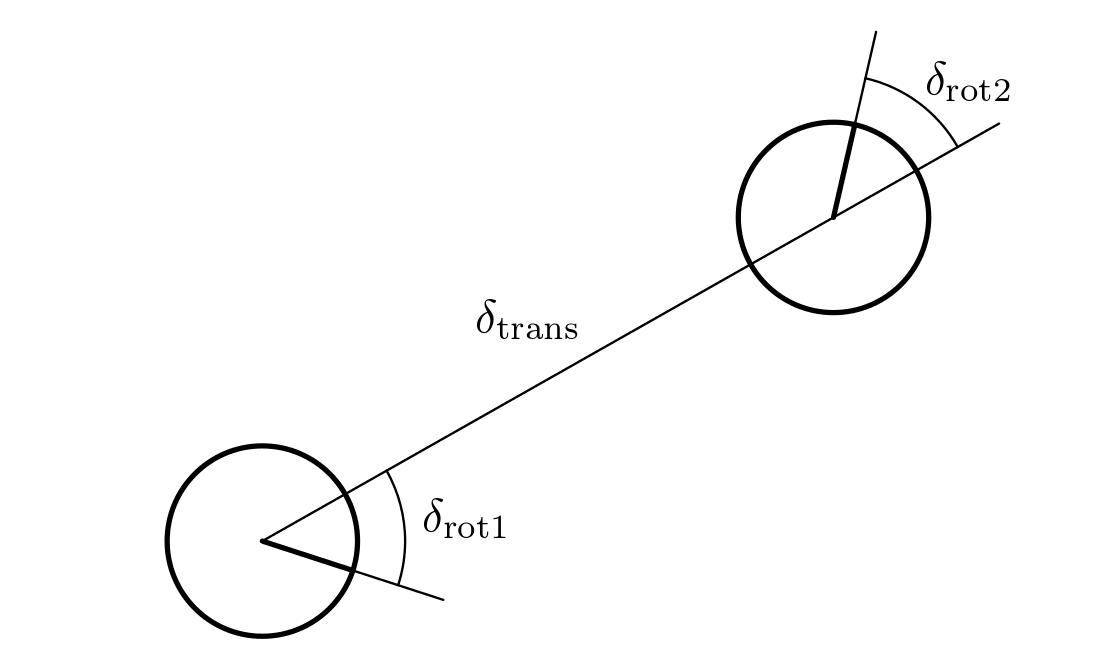
\includegraphics[scale=0.2]{./images/odometry_motion}
\caption[Approximation of robot motion in odometry model]{The robot motion is approximated by a sequence of rotation $\delta_{\text{rot1}}$, translation $\delta_{\text{trans}}$ and rotation $\delta_{\text{rot2}}$ \cite{thrun2005probabilistic}.}
\label{odometry_motion}
\end{figure}

\begin{figure}
\begin{algorithm}[H]
\caption{Sampling from odometry motion model}\label{alg_odom}
\begin{algorithmic}[1]
\BState \textbf{Input}: $s_{t-1}=[x_{t-1},y_{t-1},\phi_{t-1}]$, $[[\bar{x}_{t-1},\bar{y}_{t-1},\bar{\phi}_{t-1}],[\bar{x}_{t},\bar{y}_{t},\bar{\phi}_{t}]]$
\Procedure{Controls}{}
\State $\delta_{\text{rot1}} = {\bf atan2}(\bar{y}_{t}-\bar{y}_{t-1},\bar{x}_{t}-\bar{x}_{t-1}) - \bar{\phi}_{t-1}$
\State $\delta_{\text{trans}} = \sqrt{\strut(\bar{y}_{t}-\bar{y}_{t-1})^2+(\bar{x}_{t}-\bar{x}_{t-1})^2}$
\State $\delta_{\text{rot2}} = \bar{\phi}_{t} - \bar{\phi}_{t-1} - \delta_{\text{rot1}}$
\EndProcedure
\Procedure{Sampling}{}
\State $\hat{\delta}_{\text{rot1}} = {\bf gauss}(\delta_{\text{rot1}},\alpha_1\delta_{\text{rot1}}+\alpha_2\delta_{\text{trans}})$
\State $\hat{\delta}_{\text{trans}} = {\bf gauss}(\delta_{\text{trans}},\alpha_3\delta_{\text{trans}}+\alpha_4(\delta_{\text{rot1}}+\delta_{\text{rot2}}))$
\State $\hat{\delta}_{\text{rot2}} = {\bf gauss}(\delta_{\text{rot2}},\alpha_5\delta_{\text{rot2}}+\alpha_6\delta_{\text{trans}})$
\EndProcedure
\Procedure{Propagation}{}
\State $x_t = x_{t-1} + \hat{\delta}_{\text{trans}}\cdot{\bf cos}(\phi_{t-1}+\hat{\delta}_{\text{rot1}})$
\State $y_t = y_{t-1} + \hat{\delta}_{\text{trans}}\cdot{\bf sin}(\phi_{t-1}+\hat{\delta}_{\text{rot1}})$
\State $\phi_t = \phi_{t-1}+\hat{\delta}_{\text{rot1}}+\hat{\delta}_{\text{rot2}}$
\State \textbf{return} $s_t=[x_t,y_t,\phi_t]$
\EndProcedure
\end{algorithmic}
\end{algorithm} 
\caption[Sampling algorithm for odometry motion model]{New pose $[x_t,y_t,\phi_t]$ is sampled from old pose $s_{t-1}=[x_{t-1},y_{t-1},\phi_{t-1}]$ through a set of translation $\delta_{\text{trans}}$ and rotations $\delta_{\text{rot1}}$ and $\delta_{\text{rot2}}$. The last input is the consecutive odometry measurement from time $t-1$ to $t$.}
\end{figure}

\subsection{Observation model}   
The measurements available from the Sphero robot are odometry and collision measurements. The odometry from the IMU provides the robot pose through dead-reckoning and the correlation between the robot position from odometry and landmark position is straightforward since for the impact-based SLAM, the robot is present at the absolute location of collision (except for an offset which can be corrected in the map). The nonlinear relation between the collision information $\dfrac{a_x}{a_y}$, robot orientation $\theta$ and landmark orientation $\phi$ is shown below,
\begin{equation*}
\phi-\theta = \arctan\left(\frac{a_x}{a_y}\right)
\end{equation*}

The resulting observation model of a landmark $l$ is shown,
\begin{equation*}
y_l = \begin{bmatrix}x_r \\ y_r \\ c_r\end{bmatrix} = \begin{bmatrix}
x_l \\ y_l \\ \tan(\phi-\theta),
\end{bmatrix}
\end{equation*}
where $(x_l,y_l)$ denotes the landmark position, $(x_r,y_r)$ denotes the robot odometry and $c_r$ denotes the collision information. Note that the robot orientation $\theta$ is also a part of the measurement. A probabilistic version can be obtained from the observation model much similar to the sampling approach in motion model.
 
\section{Environment representation} \label{sec::env_rep}
A suitable environment representation is needed to build a map of the environment and use the map to estimate the robot trajectory. The accuracy of a map representation is directly correlated with the accuracy of the SLAM solution, and care is taken to represent the environment in the best possible way. 

In the case of impact-based SLAM, the given environment is an indoor world which comprises of rectilinear walls. The orthogonality assumption in walls is crucial for orientation correction for the robot. In addition, equal corridor width in the environment is a common assumption in indoor environments for correcting the position of the robot \cite{jensfelt2001approaches}. Additional assumptions such as boundary length are taken for building a map to ensure consistency if needed. 

The most suitable representations of an indoor environment are point landmarks, line representations and occupancy maps. The first is more simple than the other while the last involves more book-keeping. The later representation is more useful for the case of planning, and its variants are in use for the Google autonomous car. The line representation is suitable for a SLAM problem with a range-and-bearing sensor. The suitability of a map representation is deeply correlated with the data association (refer \ref{sec::da}) used for SLAM. Suitable environment representations for the impact-based SLAM problem are presented below.

\subsection{Point landmarks}
The point landmarks are described using pose information, or in other words, position and orientation (though mathematically, it is not appropriate for a point to be described using orientation). For the case of impact-based SLAM, the collision information has to be encoded in such a way to initialize and update corresponding landmarks for each and every collision. 

The point landmark representation is the most preferred representation in literature for analysis. The map is defined as a set of point landmarks where each landmark $m_i$ is defined by its pose and possible signatures. 
\begin{equation}
m = \begin{bmatrix}m_1 & m_2 \cdots & m_N\end{bmatrix}
\end{equation}
The simplest description of a point landmark is by its position $m_i=\begin{bmatrix}x_i & y_i\end{bmatrix}^T$. Additional components such as landmark signatures (e.g.\ color, texture) can be added to improve the description. 

For a 3-dimensional pose description of a point landmark, the uncertainty associated is also 3-dimensional in nature and can be modelled as a multivariate Gaussian.
\begin{equation}
\mathcal{N}\left(\begin{bmatrix}x_i \\ y_i \\ \phi_i \end{bmatrix},\begin{bmatrix}\sigma_{xx} & \sigma_{xy} & \sigma_{x\phi} \\ \sigma_{xy} & \sigma_{yy} & \sigma_{y\phi} \\ \sigma_{x\phi} & \sigma_{y\phi} & \sigma_{\phi\phi}\end{bmatrix}\right)
\end{equation}

For the case of impact-based SLAM problem, the use of point landmark is insufficient to completely represent the environment since the environment is rather more descriptive than point landmark representation. In addition, even if SLAM is carried out for a simple corridor environment, new landmarks are created for every collision and it is very rare that the robot touches the same landmark again. 

The above situation can however be avoided with two possible solutions-
\begin{enumerate}
\item The uncertainty associated with each landmark can be increased such that close collisions could be regarded as a single landmark. However, this can result in overestimation or a highly conservative estimate, and result in an inaccurate solution. This situation is exemplified in Example~\ref{example1}.  
\item The spatial information of the wall can be taken into account for clubbing collisions on the same wall. This technique involves taking only uncertainty along the orthogonal direction since orthogonal direction of uncertainty can be reduced from collision updates. However, the associated result was found to be poor since the environment information is not completely encoded, as exemplified in Example~\ref{example2}.
\end{enumerate}

A more suitable representation is required for a better description of the indoor environment as point landmarks were no more suitable. The data association results tend to fail a lot with these representations and hence, more complex representations are needed to better suit the environment and the algorithm. A new representation is required to suit a rectilinear environment for impact-based SLAM as well as address the issues of point landmark representation.

\begin{exmp} {\it Consider the Sphero robot mapping a corridor environment. The robot moves in a straight line between consecutive collision and the uncertainty associated with each collision is modelled as a Gaussian. The collision information is encoded as a point landmark and the associated algorithm is detailed.}

\qquad In standard EKF-SLAM, landmark pose is a component of mean of the multivariate Gaussian and associated uncertainty is maintained as sub-covariance of the Gaussian. A landmark is created from a measurement that does not correspond (nearest-neighbour gating) to any old landmark and updated if the corresponding landmark has a higher likelihood. Note that the association of point landmarks to measurements in this example holds for any data association algorithm in literature.

This approach is found to be less suitable for point landmarks since new landmarks are created for every collision within walls and there are no EKF updates. Hence, the associated uncertainty grows unbounded and there is no convergence in the solution. This can be illustrated in Figure~\ref{ex1_pl}. 

\begin{figure}
\centering
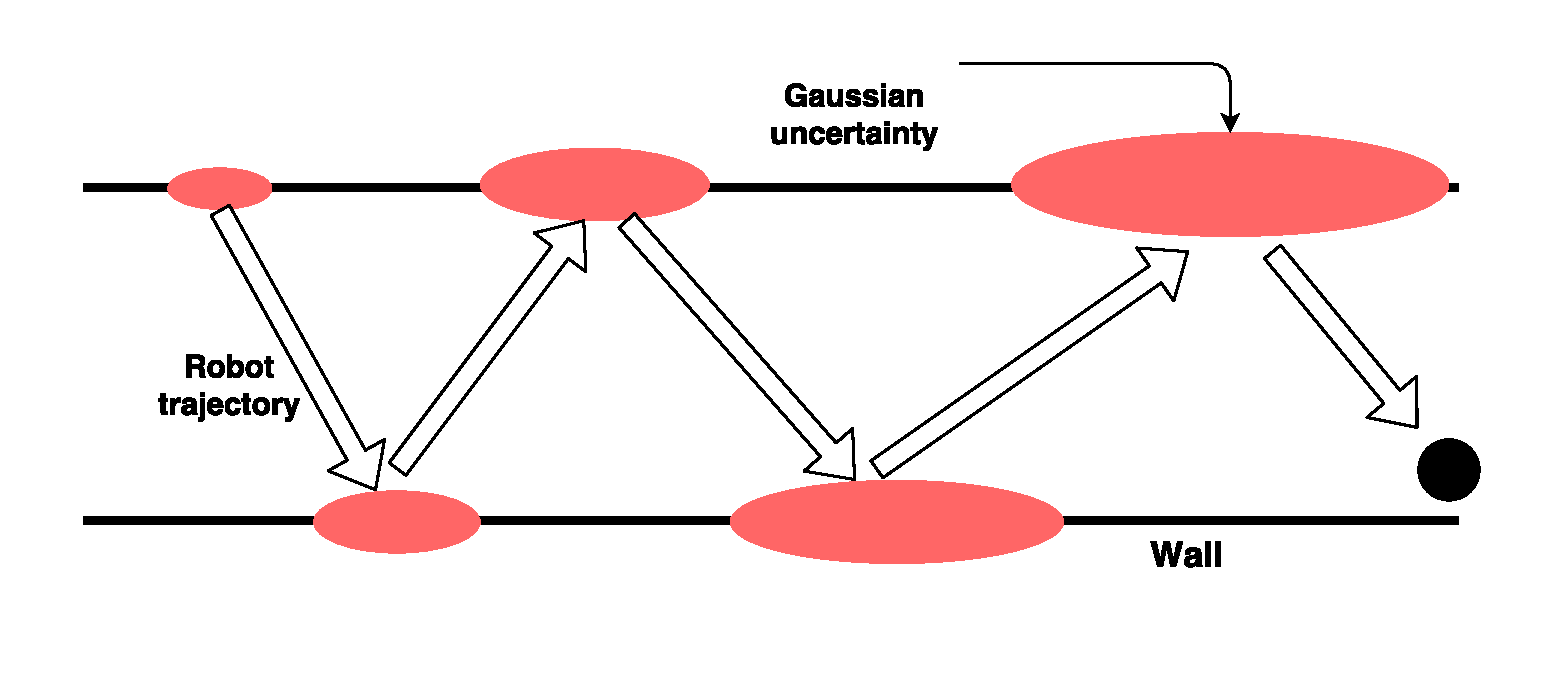
\includegraphics[scale=0.5]{./images/ex1_pointlandmark}
\caption[A simple point landmark representation]{New landmarks are created for collisions on the same wall. The robot coordinate frame is same as map coordinate frame.}
\label{ex1_pl}
\end{figure}  

In this example, five landmarks are created rather than two landmarks. The state vector of EKF-SLAM as a result becomes
\begin{equation}
x=\begin{bmatrix}x_r \\ y_r \\ \phi_r \\ m_1 \\ m_2 \\ m_3 \\ m_4 \\ m_5 \end{bmatrix}
\end{equation}

The size of state is found to increase linearly in the number of collisions and the uncertainty correspondingly grows unbounded. 

A suitable approach to overcome this issue is to go for scaled or inflated representation of uncertainty \cite{julier2003stability} such that close-by landmarks of the same wall can have lower Mahalonobis distance. The scaled representation is illustrated in Figure~\ref{ex1_scalepointlandmark} .
\begin{figure}
\centering
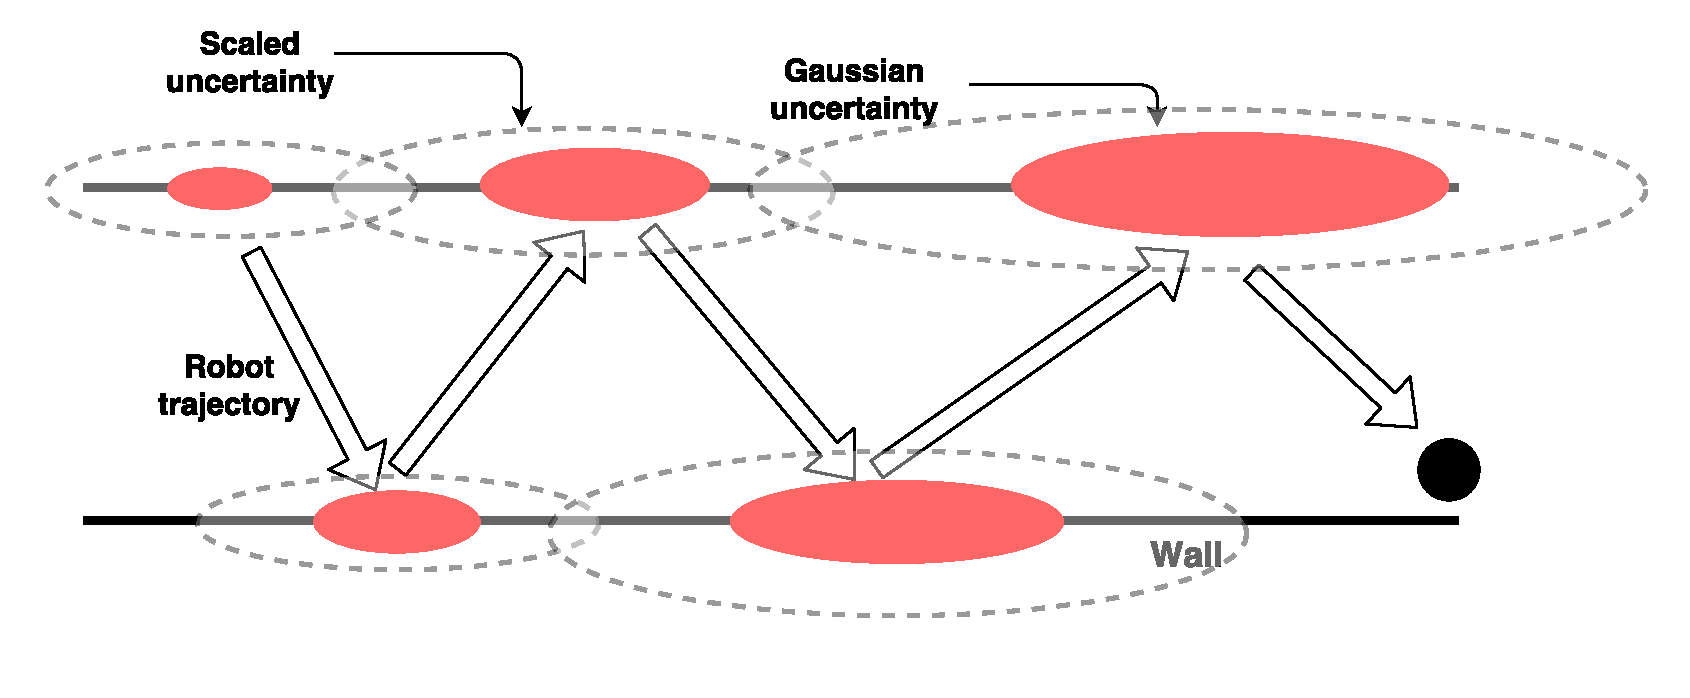
\includegraphics[scale=0.5]{./images/ex1_scalepointlandmark}
\caption[Scaled representation of point landmarks]{Scaled uncertainty to improve data association over the same wall}
\label{ex1_scalepointlandmark}
\end{figure}  

The resulting EKF-SLAM state turns out to be
\begin{equation}
x=\begin{bmatrix}x_r \\ y_r \\ \phi_r \\ m_1 \\ m_2 \end{bmatrix}
\label{eq_state}
\end{equation}

Consistency of map via this approach might be achieved by inflating the covariance \cite{julier2003stability} but it is not clear how to quantify adequate inflation. Even though the representation may appear simple, this technique may result in an unbounded growth in covariance with a non-converging solution. This is due to partiality in the uncertainty updates along the unit normal direction of the wall, which is usual in rectilinear environments.\hfill $\square$
\label{example1}
\end{exmp}

\begin{exmp} {\it Consider a similar situation to Example~\ref{example1} where the robot collides along the walls of a corridor. Spurious landmark creation were avoided by inflating the covariance matrix to ensure a consistent solution for the map. However, the map structure can be taken into account to reduce the overall scaling of the uncertainty representation.} 

\qquad A reduced state representation of the landmark state is chosen for data association. Let X-axis denote the orthogonal direction to the wall and Y-axis denote the axis along the wall. As the Y-axis correspond to the same landmark along the wall direction, collisions on the same wall (Y-axis) also correspond to the same landmark. Hence, the X-axis coordinate and orientation (reduced state) can be used for data association since the Y-axis does not contribute to any useful information for data association. This introduces a bounded covariance for this reduced state representation. The uncertainty along the wall axis (Y-axis) can be reduced when a joint covariance representation of all the landmarks are maintained or a \acf{CI} update is used between neighbouring orthogonal landmarks for incorporating orthogonal measurement information (Refer Section~\ref{sec::single_slam}).

In addition, information about the geometric structure of the environment can be incorporated. Constraints such as equal corridor width, orthogonality in wall orientation and boundary length can be incorporated into EKF as zero-uncertainty measurements \cite{newman1999structure}. Addition of these measurements can reduce the growth of covariance and ensure consistency of the SLAM solution.

The corridor width $w$ in an usual indoor environment is assumed to be constant \cite{jensfelt2001approaches}. This structure can be exploited to reduce the uncertainty along the orthogonal direction to the wall. For example, the two walls, each parametrized as a hyperplane $a_i^Tx=b_i$ where $x$ can be same as Equation \ref{eq_state}, can model the equal width constraint as
\begin{equation}
y = w = a_1^T\cdot x-a_2^T\cdot x = b_1-b_2 
\end{equation}

The orthogonal assumption and boundary length can be incorporated in a similar fashion. This technique can avoid the spurious landmark creation but at the expense of additional computation complexity through a joint covariance or constraint incorporation using covariance intersection (as detailed in the next chapter). \hfill $\square$
\label{example2}
\end{exmp}

The last approach still has an important disadvantage (Example~\ref{example1}) which is poor representation of the environment. The information of wall mass is not represented anywhere in point landmarks. For example, the spatial information (wall mass) of a discontinuous wall (as illustrated in Figure~\ref{gaussian_wall}) cannot be properly modelled as a Gaussian and it requires a more elaborate representation such as occupancy map or particles. Moreover, if distant collisions of the same wall are clubbed as a single landmark, combinatorial possibilities can open up whether they correspond to the same landmark or not during the pruning step (door openings might be present in between two collisions on the same wall). 
\begin{figure}
\centering
\begin{subfigure}{0.5\textwidth}
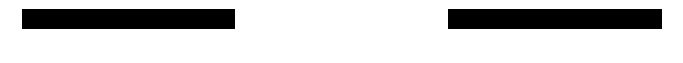
\includegraphics[scale=0.4]{./images/actual_wall.png}
\caption{A one-dimensional wall with discontinuous mass along the wall}
\end{subfigure}
\begin{subfigure}{0.5\textwidth}
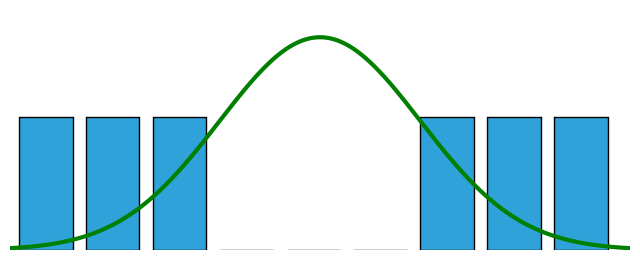
\includegraphics[scale=0.4]{./images/gaussian_wall.png}
\caption{Histogram and Gaussian representation of the wall mass}
\end{subfigure}
\caption[Spatial representation of a map information]{Spatial representation of wall mass information for a simple 1-D environment}
\label{gaussian_wall}
\end{figure}

The suitability of point landmarks for impact-based SLAM is also shown through simulations in the forthcoming chapter. 

\subsection{Occupancy maps}
A more popular and descriptive representation of a map than a point landmark is an occupancy grid where the entire map of an environment is rasterized into small cells. Each cell encodes the occupancy information and as a result, processing of information and estimation~\cite{thrun2005probabilistic} becomes more simple. For example, a cell $(i,j)$ is described by an occupancy state $x$ as,
\[ x(i,j) = \begin{cases}\,\,1 & \quad \text{if } \text{cell is occupied}\\ \,\,0 & \quad \text{if } \text{cell is free}\\ \,-1 & \quad \text{if } \text{cell is unknown} \end{cases} \] 

The occupancy map representation does not include any information about landmark signature and this map representation has been used extensively for planning and navigation since most of the planning algorithms favour a grid-structured map.

Occupancy maps can represent any arbitrary distribution at the expense of higher memory requirements. Impact-based SLAM in literature (\cite{fox2012tactile}, \cite{fox2012towards}) use an occupancy grid representation to account for the poor uncertainty distribution in impact-based mapping and SLAM. 

This thesis strikes a mid-level between a point landmark representation and occupancy map representation, by exploiting the advantages of both the approaches and aiding each other at shortcomings. Without further delay, the forthcoming section will detail the histogram representation of a map.

\subsection{Histogram maps} \label{sec::hist_map}
The thesis proposes a hybrid approach to an environment representation, much suitable for rectilinear environments. A landmark is represented using a point landmark description as well as with a histogram description. The landmark will turn out to be more descriptive than point landmarks and at the same time, the representation requires less of book-keeping compared to occupancy maps. Histogram representation of a 1D map has been used in literature \cite{thrun2005probabilistic} for pedantic purposes and not for a real-world implementation since occupancy maps turn out to be more descriptive.

Before getting deeper into histogram maps, a histogram is first defined.
\begin{defn} A histogram is a bar graph, illustrating the mapping $\mathcal{F}$ between finite domain $\mathcal{X}$ and its associated range $\mathcal{Y}=\mathcal{F}(\mathcal{X})$. A histogram can also represent a probability distribution where the domain represents a finite set of events and the range represents the associated probability of an event.
\end{defn}
Taking a more specific example (refer Figure~\ref{gaussian_wall}) such as a wall in an indoor environment for impact-based SLAM, the domain represents discretized wall location along the wall. The associated range describes the probability of mass information along the wall. To make it more clear, if X-axis describes the thickness of wall and Y-axis describes the wall length, the histogram is defined along the Y-axis and encodes information about the presence of wall. 

As said in the previous section, histogram maps strike a mid-level between point landmark representation and occupancy grid representation. For an indoor environment, each wall is described as a point oriented landmark where its pose is determined from the initial collision which lead to its inception. As a new landmark gets created, a new state describing its pose is augmented to the system state. In addition to the new state, a histogram with a finite support is also initialized for the corresponding landmark. The length of support is taken from the prior knowledge of the size of the environment. If the size of the environment is not perfectly known, an approximate bound is taken for the size and pruned later for a consistent map. 

Figure~\ref{gaussian_wall} illustrates the histogram representation of a discontinuous wall. The histogram can represent any discontinuous, non-Gaussian distribution and shares similarities with occupancy maps. This representation is aptly suited for impact-based SLAM since the collision information can be encoded into the histogram by propagating it through discrete Bayes filter while landmark pose is propagated using EKF similar to previous point representation. The discrete Bayes filter is a simple extension of continuous Bayes filter (refer Equation~\ref{bayes_filter}) where the integral gets converted to a finite sum. Spurious landmark creation is avoided using the approach followed in Example~\ref{example2}. The propagation of a histogram using discrete Bayes filter for an impact-based SLAM problem is shown in Example~\ref{ex24}.

\begin{exmp}
{\it Consider a wall in an one-dimensional world which contains an opening (open door). This can be illustrated in Figure~\ref{wall_example3}. A robot equipped with touch sensors, can move back and forth along the wall and make contacts at certain points. In addition, the position of a robot is given by a noisy odometry. A simple assumption is made here that there is no measurement noise associated with the touch sensors.}
\begin{figure}[H]
\centering
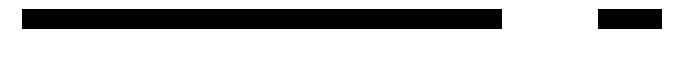
\includegraphics[scale=0.45]{./images/wall_example3.png}
\caption[A simple 1-D wall for impact-based mapping]{One-dimensional wall for impact-based mapping}
\label{wall_example3}
\end{figure}

\qquad The histogram is propagated as a probability distribution using discrete Bayes filter with a sequence of incoming measurements. The histogram represents the probability of occupancy along the wall and hence the initial distribution is assumed to be uniform. Two possible implementations of a collision update are Gaussian update and triangular update where the probability is computed at discrete points using these distributions. 

It is not necessary that histogram has to be declared as a probability distribution and use discrete Bayes' theorem for mapping the wall. A simple histogram update can be used where each cell contains a probability of occupancy (much similar to occupancy maps). Both the approaches of histogram representation have the same computational efficiency. Moreover, maintaining a collinear histogram also improves the consistency of the estimate along the wall. Figure~\ref{ex24coll_10} gives the difference between the two histogram update techniques for a single collision.

\begin{figure}
\centering
\begin{minipage}{0.45\textwidth}
\centering
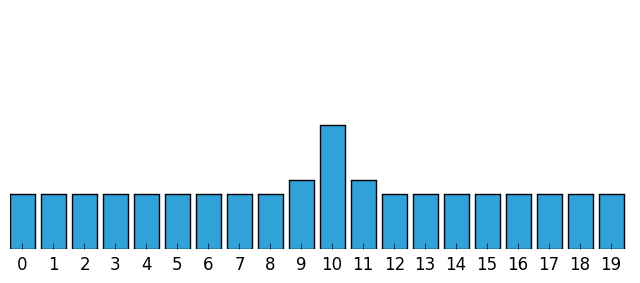
\includegraphics[scale=0.4]{./images/ex24/ex24coll10.png}
%\caption{Histogram as a probability distribution}
\end{minipage}
\begin{minipage}{0.45\textwidth}
\centering
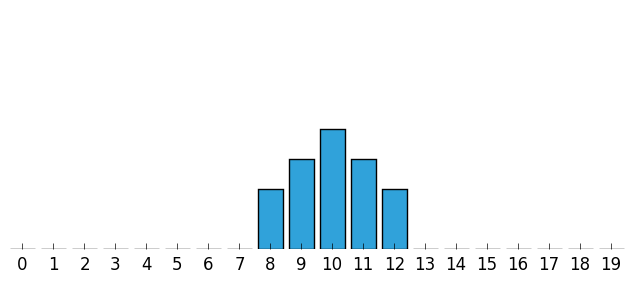
\includegraphics[scale=0.4]{./images/ex24/ex24coll10_1.png}
%\caption{A simple histogram update}
\end{minipage}
\caption[Histogram propagation of measurement information]{Propagation of histogram for an incoming measurement. The left histogram is propagated as a probability distribution whereas the right is a simple histogram update (not a probability distribution).}
\label{ex24coll_10}
\end{figure}

Figure~\ref{ex24_collisions} give a list of histogram updates along the wall, with collisions occurring according to the cell sequence $\left\lbrace 10,4,12,13,1,5,9,6,7,19\right\rbrace$. A triangular collision update is used here for simplicity. The corresponding map of the wall is shown for each collision based on the simple histogram update (for a good illustration of map formation). 

\begin{figure}
\centering
\begin{minipage}{0.48\textwidth}
\centering
\begin{subfigure}{\textwidth}
\centering
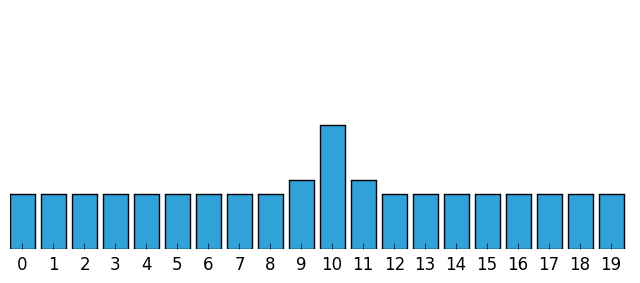
\includegraphics[scale=0.4]{./images/ex24/ex24coll10.png}
\end{subfigure}
\begin{subfigure}{\textwidth}
\centering
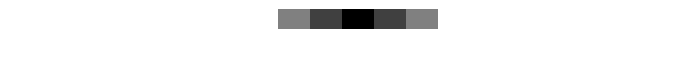
\includegraphics[scale=0.4]{./images/ex24/ex24wall10.png}
\caption{First collision at 10 and the resulting map}
\end{subfigure}
\end{minipage}
\begin{minipage}{0.48\textwidth}
\centering
\begin{subfigure}{\textwidth}
\centering
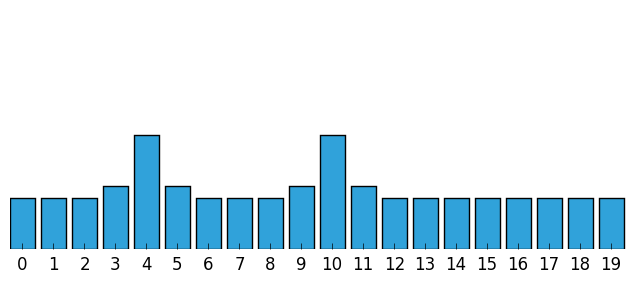
\includegraphics[scale=0.4]{./images/ex24/ex24coll4.png}
\end{subfigure}
\begin{subfigure}{\textwidth}
\centering
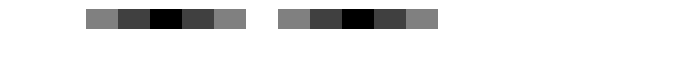
\includegraphics[scale=0.4]{./images/ex24/ex24wall4.png}
\caption{Next collision at 4 and the resulting map}
\end{subfigure}
\end{minipage}

\begin{minipage}{0.48\textwidth}
\centering
\begin{subfigure}{\textwidth}
\centering
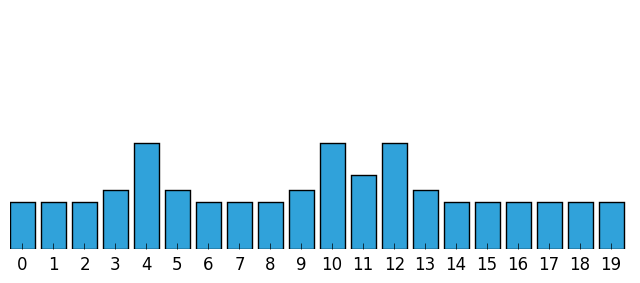
\includegraphics[scale=0.4]{./images/ex24/ex24coll12.png}
\end{subfigure}
\begin{subfigure}{\textwidth}
\centering
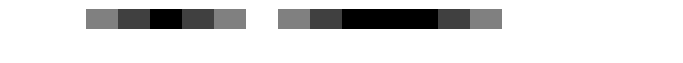
\includegraphics[scale=0.4]{./images/ex24/ex24wall12.png}
\caption{Next collision at 12 and the resulting map}
\end{subfigure}
\end{minipage}
\begin{minipage}{0.48\textwidth}
\centering
\begin{subfigure}{\textwidth}
\centering
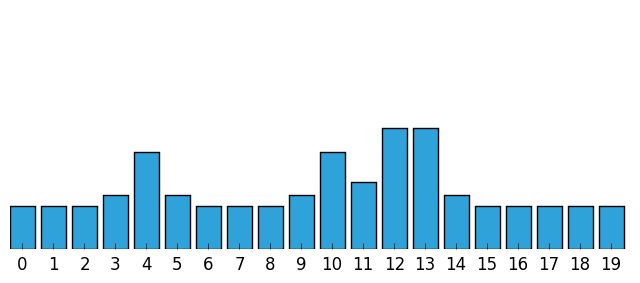
\includegraphics[scale=0.4]{./images/ex24/ex24coll13.png}
\end{subfigure}
\begin{subfigure}{\textwidth}
\centering
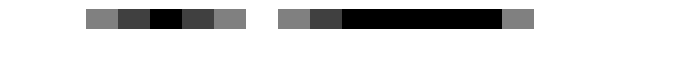
\includegraphics[scale=0.4]{./images/ex24/ex24wall13.png}
\caption{Next collision at 13 and the resulting map}
\end{subfigure}
\end{minipage}

\begin{minipage}{0.48\textwidth}
\centering
\begin{subfigure}{\textwidth}
\centering
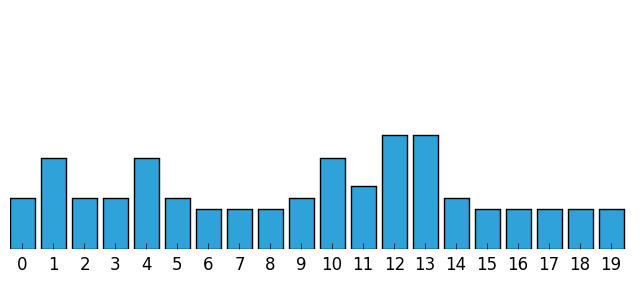
\includegraphics[scale=0.4]{./images/ex24/ex24coll1.png}
\end{subfigure}
\begin{subfigure}{\textwidth}
\centering
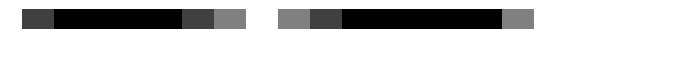
\includegraphics[scale=0.4]{./images/ex24/ex24wall1.png}
\caption{Next collision at 1 and the resulting map}
\end{subfigure}
\end{minipage}
\begin{minipage}{0.48\textwidth}
\centering
\begin{subfigure}{\textwidth}
\centering
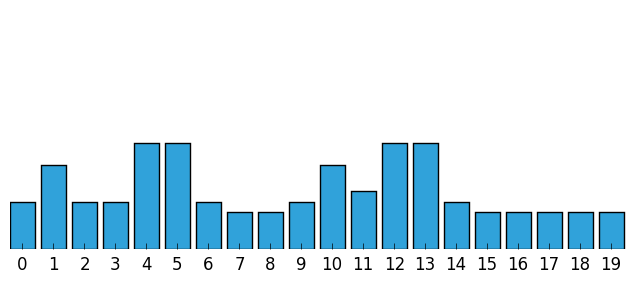
\includegraphics[scale=0.4]{./images/ex24/ex24coll5.png}
\end{subfigure}
\begin{subfigure}{\textwidth}
\centering
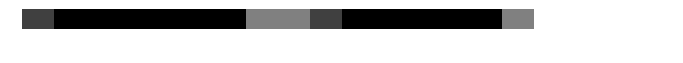
\includegraphics[scale=0.4]{./images/ex24/ex24wall5.png}
\caption{Next collision at 5 and the resulting map}
\end{subfigure}
\end{minipage}

\begin{minipage}{0.48\textwidth}
\centering
\begin{subfigure}{\textwidth}
\centering
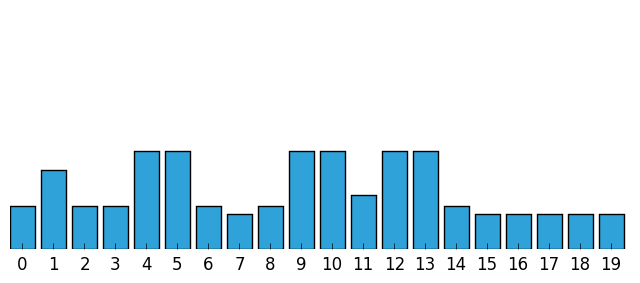
\includegraphics[scale=0.4]{./images/ex24/ex24coll9.png}
\end{subfigure}
\begin{subfigure}{\textwidth}
\centering
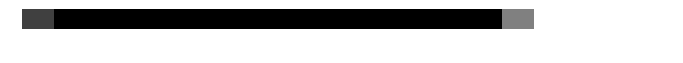
\includegraphics[scale=0.4]{./images/ex24/ex24wall9.png}
\caption{Next collision at 9 and the resulting map}
\end{subfigure}
\end{minipage}
\begin{minipage}{0.48\textwidth}
\centering
\begin{subfigure}{\textwidth}
\centering
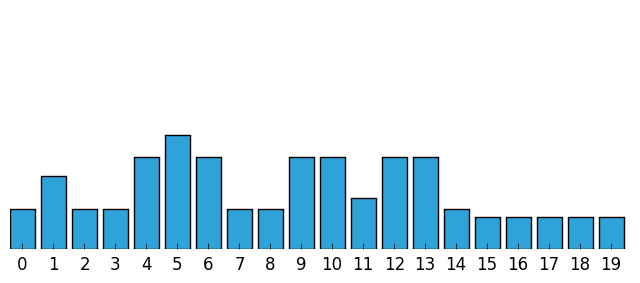
\includegraphics[scale=0.4]{./images/ex24/ex24coll6.png}
\end{subfigure}
\begin{subfigure}{\textwidth}
\centering
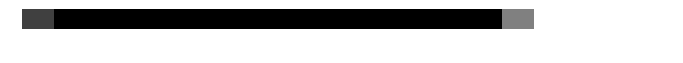
\includegraphics[scale=0.4]{./images/ex24/ex24wall6.png}
\caption{Next collision at 6 and the resulting map}
\end{subfigure}
\end{minipage}

\begin{minipage}{0.48\textwidth}
\centering
\begin{subfigure}{\textwidth}
\centering
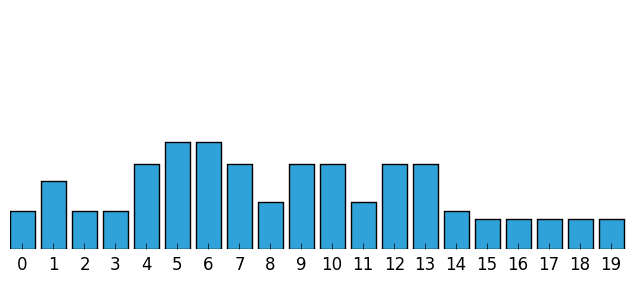
\includegraphics[scale=0.4]{./images/ex24/ex24coll7.png}
\end{subfigure}
\begin{subfigure}{\textwidth}
\centering
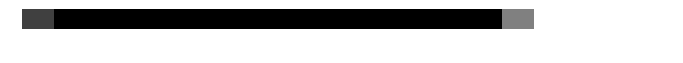
\includegraphics[scale=0.4]{./images/ex24/ex24wall7.png}
\caption{Next collision at 7 and the resulting map}
\end{subfigure}
\end{minipage}
\begin{minipage}{0.48\textwidth}
\centering
\begin{subfigure}{\textwidth}
\centering
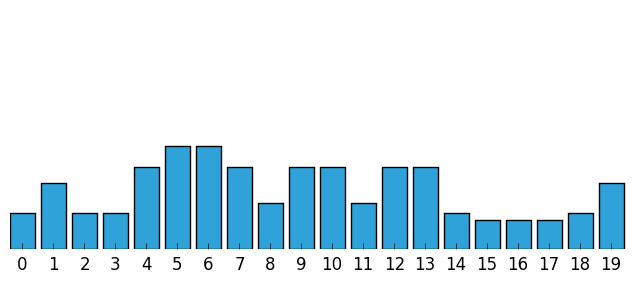
\includegraphics[scale=0.4]{./images/ex24/ex24coll19.png}
\end{subfigure}
\begin{subfigure}{\textwidth}
\centering
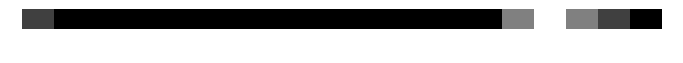
\includegraphics[scale=0.4]{./images/ex24/ex24wall19.png}
\caption{Last collision at 19 and the resulting map}
\end{subfigure}
\end{minipage}
\caption[Histogram propagation for a sequence of collision information]{Histogram propagation for a sequence of collisions}
\label{ex24_collisions}
\end{figure}

In the case the robot passes through an open door and returns back, a simple negative update is added. This update is illustrated in Figure~\ref{ex24_coll15}. \hfill $\square$
\begin{figure}
\centering
\begin{subfigure}{\textwidth}
\centering
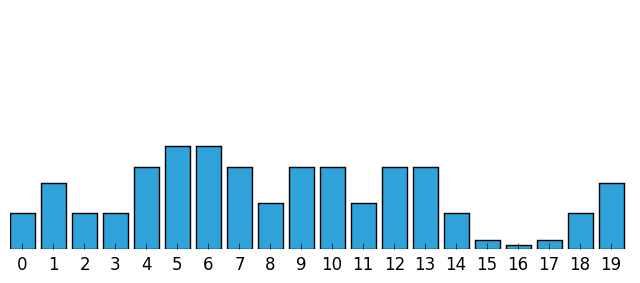
\includegraphics[scale=0.4]{./images/ex24/ex24coll15.png}
\end{subfigure}
\begin{subfigure}{\textwidth}
\centering
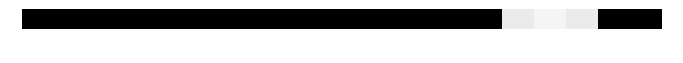
\includegraphics[scale=0.4]{./images/ex24/ex24wall15.png}
\end{subfigure}
\caption[Update of negative information in histogram]{Negative update of histogram at 15 and the resulting map}
\label{ex24_coll15}
\end{figure}
\label{ex24}
\end{exmp}   

\section{Challenges} \label{sec::challenges}
There are few challenges playing a key role to the success of a SLAM solution which limit the applicability based on robot sensors and mapping environment. Among the following challenges, lack of observability is a key fundamental limitation to state estimation in a generic SLAM. In a usual SLAM estimation, observability is presumed (with knowledge of few absolute locations) and hence it has to be made sure that the impact-based SLAM satisfies the observability property as well. Other crucial factors are data association, computational effort and consistency of estimates. The computational issues related to state-of-the-art SLAM estimation have been addressed in Section~\ref{sec::ekfslam} of Chapter~\ref{chap::intro}. 

\subsection{Observability}
Observability is a key property to be satisfied for any successful state estimation. SLAM is a nonlinear-coupled problem and hence simple linear analysis tools fail to explain the observability of SLAM. It is apparent from process model (Equation~\ref{proc_model}) is nonlinear and coupled. This also holds true for the odometric motion model where the nonlinear and coupled nature is introduced through the collision measurement equation (Equation~\ref{measurement_eq}). 

To determine the observability criterion for a general nonlinear coupled system, let us consider a smooth nonlinear system,
\begin{align*}
\dot{x} &= f(x)+\sum_{j=1}^m g_j(x)\cdot u_j, \hspace{1cm} u=col(u_1,\dots,u_m)\in\mathcal{R}^m\\
y_i &= h_i(x), \hspace{1cm} i\in p
\end{align*}
where $h=col(h_1,\dots,h_p):\mathcal{R}^n\rightarrow\mathcal{R}^p$ is a smooth output map or vector field of the system. 

The concept of observability is linked to \textit{indistinguishability} of a state since the effect of control inputs play a role in nonlinear observability. Before defining observability, the definition of \textit{indistinguishability} is first laid out.

\begin{rem}
Two states $x_1$ and $x_2$ are $\mathrm{V}$-distinguishable if there exists an input which drives system trajectories from both $x_1$ and $x_2$ remain in $\mathrm{V}$ such that the output functions are distinguishable $h(x_1)\neq h(x_2)$. Otherwise, the states $x_1$ and $x_2$ are $\mathrm{V}$-indistinguishable.
\end{rem}

The system is said to be locally observable if it can instantaneously distinguish a state from its neighbours. A rank condition test is used to determine the local observability of a given system, as shown below,
\begin{equation}
span(\mathcal{O}) = span(\begin{bmatrix}dh_1(x_0),\dots,dh_p(x_0),dL_{v_k}L_{v_{k-1}}\cdots L_{v_1}h_j(x_0)\end{bmatrix}) = n,
\end{equation}
where $v_i,i\in k$ is a vector field in the set $\left\lbrace f,g_1,\dots,g_m\right\rbrace$ and $L_{v_i}h_j$ is the Lie derivative of $h_j$ along the vector field $v_i$.

For a world-centric impact-based SLAM problem, the system state can be represented as,
\begin{equation}
x=\begin{bmatrix}x_r & y_r & \psi_r & x_l & y_l & \psi_l\end{bmatrix},
\end{equation} 
where first three variables represent the robot pose (position $x$ and $y$, orientation $\psi$) while the latter represents the landmark pose.

The representation included a single feature and can be generalized for observing as many features as possible. Using the process (unicycle) model,
\begin{align}
\dot{X}&=\frac{d}{dt}\begin{bmatrix}x_r & y_r & \psi_r & x_l & y_l & \psi_l\end{bmatrix}^ T \nonumber \\
&=\begin{bmatrix}\cos\psi_r & \sin\psi_r & \tan(\alpha)/L & 0 & 0 & 0 \end{bmatrix}^Tv, \label{proc_model}
\end{align}
where \lsymb{$v$}{Robot velocity control} and \gsymb{$\alpha$}{Robot heading control} represent the robot velocity and heading angle respectively. $L$ denotes the wheel base length.

For the impact-based SLAM problem, the odometry as measurement gives the position and orientation of the robot. A nice feature about impact-based SLAM is that at the instant of collision, the absolute location of landmark is the same as the absolute location of the robot. The measurement function as a result has a diagonal structure which makes the Jacobian computation and observability analysis easier.

The observation of a landmark given the robot and observed landmark pose is,
\begin{equation}
y_l = \begin{bmatrix}x_r \\ y_r \\ c_r\end{bmatrix} = \begin{bmatrix}
x_l \\ y_l \\ \tan(\psi_l-\psi_r),
\end{bmatrix}
\label{measurement_eq}
\end{equation}
where $y_l$ is the expected sensor measurement of the $l^{\text{th}}$ landmark. The measurement $c_r$ is a analytical expression obtained through the geometry of robot impact against a rectilinear wall.

By taking zero-order Lie derivatives, we can get the rank condition satisfied assuming the initial condition of the system or initial robot pose is known.
\begin{equation}
\mathcal{O}=\begin{bmatrix}
1 & 0 & 0 & 0 & 0 & 0 \\
0 & 1 & 0 & 0 & 0 & 0 \\
0 & 0 & 1 & 0 & 0 & 0 \\
0 & 0 & 0 & 1 & 0 & 0 \\
0 & 0 & 0 & 0 & 1 & 0 \\
0 & 0 & -s^2 & 0 & 0 & s^2 \\
& & \vdots & &  &
\end{bmatrix}
\end{equation}

The rank condition is satisfied with $rank(\mathcal{O})=6$. The result can be generalized for observation of as many landmarks as possible. $s^2$ represents $\sec^2(\psi_l-\psi_r)$ which is the derivative of measurement equation.

However, there is a downside to the impact based mapping for SLAM. At the instant of collision, the robot is touching the wall which makes the assumption of a smooth pose distribution invalid. The resulting pose distribution can only be represented by a set of particles which makes particle filter most suitable for localization. This is because the landmark (covariance) representation has to be consistent with the current robot pose (covariance) representation at the point of collision and this has to hold vice-versa. This fundamental representation of probability distribution must hold true for propagation of pose and landmark estimates to ensure consistency in estimation. Figure~\ref{robot_wall} illustrates the representation of probability distribution for impact-based approach to mapping.

\begin{figure}
\centering
\begin{subfigure}{0.3\textwidth}
\centering
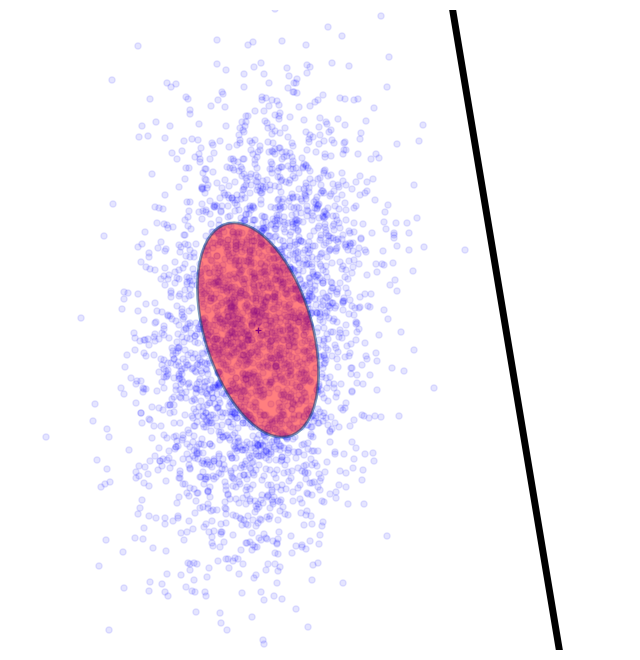
\includegraphics[scale=0.25]{./images/wall_robot.png}
\caption{}
\label{wall_robota}
\end{subfigure}
\begin{subfigure}{0.3\textwidth}
\centering
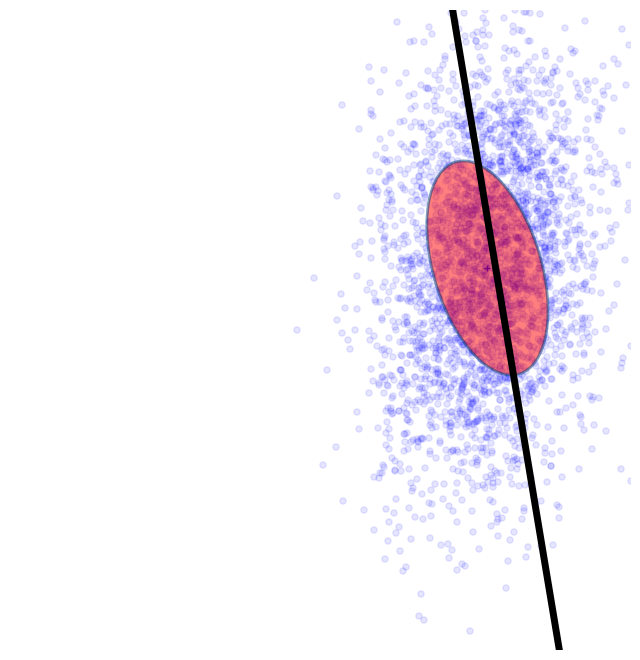
\includegraphics[scale=0.25]{./images/wall_onrobot.png}
\caption{}
\label{wall_robotb}
\end{subfigure}
\begin{subfigure}{0.3\textwidth}
\centering
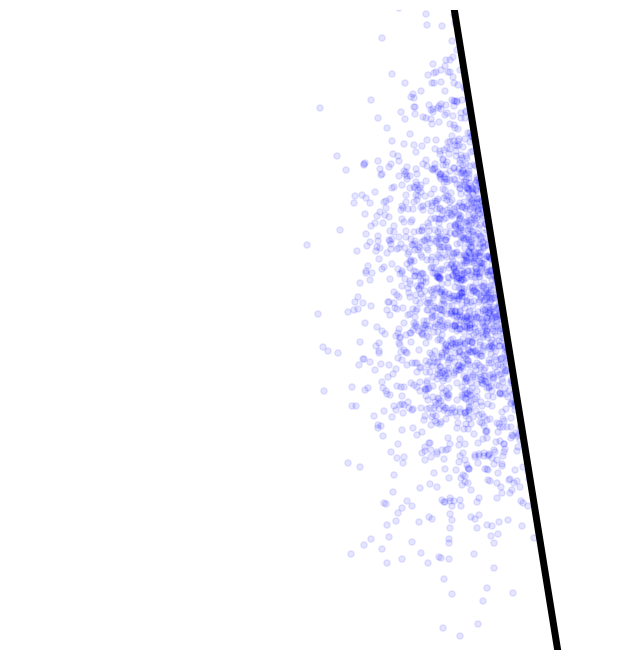
\includegraphics[scale=0.25]{./images/wall_robotp.png}
\caption{}
\label{wall_robotc}
\end{subfigure}
\caption[Gaussian and particle representation of robot pose distribution]{\subref{wall_robota} Gaussian and sampled representation of robot pose uncertainty moving towards a wall, \subref{wall_robotb} Gaussian and sampled representation of robot pose uncertainty for colliding against the wall, \subref{wall_robotc} Sampled representation of pose uncertainty taking wall constraints into account}
\label{robot_wall}
\end{figure} 

\subsection{Correlation and Consistency} \label{sec::conscorr}
The correlation through robot pose error has been considered a crucial factor in the SLAM problem since it has contributed to the tractability of the problem. However, the problem of introducing uncertainty as a bridging factor between localization and mapping has their own ups and downs. 

The main advantage, as mentioned, is the tractability in solving the SLAM problem since it can be used to improvise the robot pose estimate through reobservation of old landmarks. The robot tries to correct its pose and simultaneously improves the pose of all the previously observed landmarks due to the common correlation in the observations. The solutions dealing with explicit correlations are shown to be successful in practical implementations \cite{durrant2006simultaneous}. The representation of correlations through uncertainty information has led to the popularity of the probabilistic methods in SLAM.      

However, there is a downside to the use of robot uncertainty (process noise) in the problem as the bridging factor. The effect of using uncertainty to influence the observability in the problem has a dig at the consistency of the estimation. To improve the convergence of the solution to the problem, the correlation have to improve with time, or said in other words, higher the correlation, better is the SLAM. The problem is that increase in uncertainty, if not properly modelled in SLAM, can be really problematic since it can lead to optimistic estimates of the uncertain state variables which cannot be compensated unlike in usual tracking and navigation problems.  

Before getting into the problems of consistency due to the structure and assumptions in SLAM, the definition \cite{julier2001counter} is first laid out.
\begin{defn}
An estimator is said to be consistent if the estimated state converges to the true value and remains thereon unless an external disturbance acts on it. If $e_n$ is the error in the estimate, the true covariance or variation in the actual system state can be written as $E(e_n^Te_n)$. $\Sigma_n$ is the estimated covariance or estimated variation of error in the system. 

Mathematically, an unbiased estimator is consistent if and only if it can capture the true variation in error. 
\begin{equation}
\Sigma_n=E(e_n^Te_n)
\end{equation} 
\end{defn}

However, this condition of consistency is difficult to establish due to the stochastic scenario of a system. To enforce consistency, conservativeness is introduced so that we can bound the true variation of error at all time instances. Mathematically,
\begin{equation}
\Sigma_n-E(e_n^Te_n)\geq 0
\end{equation} 

A standard solution to ensure consistency is to inflate the observation covariance by padding it with sufficiently large values. This process is called as ``covariance inflation'' or injection of stabilizing noise into the system \cite{julier2003stability}. There is however a problem associated with this technique. Due to the inflation of noise covariance, the assumed uncertainties in certain directions of state space increases and as a result, the steady state covariance can grow unbounded.

Consistency in the SLAM scenario can be discussed based on the estimator or optimization technique to be implemented for the SLAM problem. The question of consistency can raise from several issues related to the SLAM problem such as data association errors, modelling errors, transformation errors.

The effect of data association is highly sensitive and a single incorrect association will lead to inconsistency in the solution. The first issue has been addressed a lot in the literature \cite{cooper2005comparison} and is detailed for the impact-based SLAM problem in the next section. The effect of inconsistency due to probability transformation errors have been studied and suitable solutions are developed in \cite{julier2004unscented}. The inconsistency issues relevant to EKF-SLAM and particle filter-SLAM are discussed below.

\subsubsection{EKF-SLAM}
The structure and properties of the Extended Kalman Filter-SLAM, as discussed previously, will be revisited to discuss about source and effects of inconsistency. The inconsistency in EKF-SLAM arises from linearization error in observation and inverse observation models.

To ensure consistency, the following condition \cite{julier2001counter} has to be satisfied,
\begin{equation}
\nabla h_s - \nabla h_{m_i}\nabla g_s = 0
\end{equation}
where $\nabla h_s$, $\nabla h_{m_i}$ represent the Jacobian of the measurement function with respect to robot state and landmark estimate respectively. $\nabla g_s$ denotes the Jacobian of inverse measurement function with respect to the state. Usually, this function is never satisfied due to linearization errors and as a result, the estimates turn inconsistent. As the relationship depends upon the nonlinear system models and noisy state estimates, the linearization error is difficult to compute and cannot be compensated through inflation of error covariance. 

The effect of linearization errors can be reduced through local map fusion which uses the robot's local coordinate frame to update the map \cite{castellanos2007robocentric}. This approach has a lower error in the state estimates which in turn reduces the effect of inconsistency. The use of multiple robots in impact-based SLAM ensures a higher consistency in the local map updates which can be later merged. Other approaches such as observability constrained estimation \cite{huang2011observability} also ensures a more consistent state estimation at every time step.

\subsubsection{Particle filter-SLAM}
An advantage about the use of particle filters is elimination of inconsistency due to probability transformation errors since the particle set can be propagated through any nonlinear model. 

However, there are two other key issues related to inconsistency in particle filter-SLAM. The first issue is inconsistency through modelling errors and the second i degeneracy in the estimation process.

The particle filter-SLAM problem exploits the Rao-Blackwellized property where landmark estimation problems are conditional independent given the robot trajectory. This property is based on on the assumption that the environment is unstructured, or in other words, the environment contains randomly placed landmarks. The only correlation factor is the robot pose error in the SLAM problem which is conditioned to make the landmark estimation independent. However, in the case of a rectilinear environment, the landmarks are correlated through the geometric symmetry in the environment such as orthogonal walls. Hence, a straightforward implementation of Rao-Blackwellized particle filter to SLAM problem results in inconsistent estimation. 

The effect of cross-correlations cannot be ignored since they are crucial for ensuring consistency in the SLAM estimation. The lack of proper correlations leads to a poor covariance estimate which leads to inconsistency (refer Remark~\ref{rem_corr}). The cross-correlations in the environment can be effectively maintained using a joint covariance matrix (a single EKF for all the landmarks) for every particle in the particle set. This approach might lead to computational issues since every measurement update requires a computation complexity of $\mathcal{O}(M\cdot N^2)$ which is cumbersome.

A more computationally efficient approach is to conservatively incorporate the conditionally independent landmarks (through Rao-Blackwellization) with the orthogonality and partial uncertainty constraints through \acf{CI} technique \cite{julier2007using}. This approach ensures a consistent estimation in a conservative fashion at the expense of optimal performance (rate of map convergence). With this approach, the computational efficiency of Rao-Blackwellization is still maintained.

For the case of degeneracy, the particle filter-SLAM produces optimistic uncertain estimates in the long term, \cite{bailey2006consistency}. In general, particle filters provide a consistent recursive estimation through resampling in situations where a system exponentially forgets its past estimate errors. The problem in particle filter-SLAM is that the past pose errors are never forgotten since they are recorded in the map estimates through correlations and each time a resampling is performed, the particle that is not selected gets thrown out with an entire map hypothesis. Hence, the particle filter degenerates a good knowledge of map hypotheses and the most likely particle (with largest importance weight) duplicates by replacing other unlikely particles in the resampling step. 

As a result, there is a variance reduction in the particle set which can result in an underestimated covariance. The algorithm starts to get optimistic about the uncertainty in the trajectory of the robot and the landmark locations. Every time a particle is lost due to resampling, an entire map hypothesis is lost and there is a depletion of historical information. Hence, the overall map statistics degrade and the algorithm finds it difficult to close larger loops. Moreover with the loss of past information, data association errors cannot be corrected based on the future measurements which brings brittleness in data association similar to standard EKF-SLAM.

In the short term, particle filter-SLAM might produce consistent results given a sufficient number of particles. To avoid this problem, adaptive resampling techniques are adopted to ensure long term consistency in the solution. In addition, impact-based SLAM have sparse measurements with frequent loop closures (in corridors) which might result in degeneracy. This can be avoided through the inclusion of measurements in the prediction step, resulting in a more consistent estimate with less number of particles. Section~\ref{sec::fastslam_pred}~and~\ref{sec::fastslam_resample} detail the modified prediction step and and adaptive resampling techniques for the impact-based SLAM problem.

\subsection{Data Association} \label{sec::da}
Data association determines the mapping from the measurements to the landmarks and it is one among the essentials for achieving a successful SLAM solution. The association is quite sensitive to the uncertainty of robot involved in SLAM and few incorrect associations can lead to inconsistency in the SLAM estimation. Over the past years, this issue has been dealt seriously and robust data association techniques were developed to ensure consistency.

The data association algorithm depends upon the characteristics of landmarks and availability of measurements. Two of the most popular approaches for data association are \acf{ML} and \acf{JCBB} \cite{bailey2006simultaneous}, former being the simplest and vulnerable one.  The later approach is most useful for a SLAM where batch measurements are available for processing at each time instant. Apart from the two approaches, Multiple Hypotheses data association \cite{jensfelt2001active} has been the most accurate of all but with a computational burden of maintaining all the possible associations of landmarks with measurements.  

For impact-based SLAM using particle filter, each particle maintains a copy of the map and hence, data association decisions can be made on a per-particle basis. This leads to a robust multiple hypothesis association. The particles are not only a representation of uncertainty of state estimate but are also individual hypothesis of the map. Hence, Multiple Hypotheses is ingrained in the particle filter-SLAM formulation.

Among the data association algorithms, the most suitable one is \acf{ML} association where each particle performs a ML association for the incoming measurements. 

\begin{rem}
In data association, following assumptions have to be considered for an analytical representation of landmark likelihood to a measurement.
\begin{enumerate}
\item The incoming measurements are normally distributed, i.e., the measurement noise is Gaussian
\item Knowledge of the Gaussian parameters, mean and standard deviation, are available a-priori 
\end{enumerate}
\end{rem}

The data association is computed using likelihood function, also known as $\chi^2$ test. The maximum likelihood problem is posed as shown below,
\begin{equation}
d_l = \arg\max_{j}\frac{1}{\left(2\pi\right)^{n/2}\cdot\sqrt{\strut S_j}}\exp\left(-\frac{1}{2}e_{ij}^T\cdot S_j^{-1}\cdot e_{ij}\right),
\label{da_pfslam}
\end{equation}
where $d_l$ is the $l^{\text{th}}$ data association for measurement $i$ and landmark $j$. The variable $e_{ij}$ is the innovation vector for the pair $\left\lbrace i,j\right\rbrace$ pair, $S_j$ is the innovation covariance matrix and $n$ is defined as the dimension of the innovation vector.

\begin{rem}
The solution can also be computed through log-likelihood for numerical stability. This approach is more suitable for data associations over multiple measurements or smoothing process in the estimation process.
\end{rem}

In the case of multiple measurements or smoothing process, the measurements are considered as a vector and are assumed to be independent. Hence, the likelihood is defined as joint probability, which under the measurement independence assumption, factor into a product of marginal probabilities and the magnitude of the likelihood can be quite small, often very close to zero. With a large number of observations, this value can approach the machine zero of the computing device used, leading to numerical problems. Log-transforming all these probabilities will convert these small numbers into negative numbers thus eliminating numerical instability. The solution however still remains to be the same due to the increase monotonicity of the log-function.

Taking logarithm over the likelihood, the problem is rewritten as shown below.
\begin{equation}
d_l = \arg\max_{j}\left(-\frac{1}{2}e_{ij}^T\cdot S_j^{-1}\cdot e_{ij}+\ln\left(\frac{1}{\left(2\pi\right)^{n/2}\cdot\sqrt{\strut S_j}}\right)\right)
\end{equation}

An equivalent normalized-minimization problem can also be posed as follows,
\begin{equation}
d_l = \arg\min_{j}\left(e_{ij}^T\cdot S_j^{-1}\cdot e_{ij}+\ln(|S_j|)\right).
\end{equation}

\textbf{Summary} 
In this chapter, a probabilistic formulation of the impact-based SLAM problem is laid out from the perspective of online estimation. Two robot motion models are described using a unicycle model framework for the SLAM problem. Suitable environment representations are studied for the impact-based SLAM along with the proposed histogram map. Various challenges such as observability, correlations, consistency and data association are addressed from the viewpoint of impact-based SLAM.